\documentclass[11pt, a4paper]{article}

\usepackage{natbib}
\usepackage{type1cm}
\usepackage{amsfonts, amssymb, amsmath}
\usepackage{enumerate} % import for the form like line 643
\usepackage{caption}
\usepackage{subcaption}

\usepackage{tikz}
\usetikzlibrary{shapes, arrows}
\usetikzlibrary{matrix, positioning, chains}

\usepackage{microtype}
\usepackage{bookmark}
\usepackage{hyperref}

% begin{declare}

\title{Recursive Functions of Symbolic Expressions and Their Computation by
  Machine, Part I}
\author{John McCarthy}
\date{April 1960}

\tikzstyle{box} = [rectangle, minimum width = 16, minimum height = 16, draw =
  black, text centered]
\tikzstyle{textarea} = [rectangle, minimum height = 16, text centered]
\tikzstyle{textbox} = [rectangle, minimum height = 16, draw = black, text
  centered]

\tikzstyle{pi} = [
  rectangle, rounded corners,
  minimum width = 16, minimum height = 16,
  draw = black, text centered
]

\tikzstyle{none-line} = [-, draw = none]

% end{declare}

\begin{document}

\pagenumbering{alph}
\maketitle
\thispagestyle{empty}
\pagebreak

\pagenumbering{roman}
\tableofcontents
\pagebreak
\pagenumbering{arabic}

\section{Introduction}

A programming system called LISP (for LISt Processor) has been developed for the
IBM 704 computer by the Artificial Intelligence group at M.I.T. The system was
designed to
facilitate\footnote{facilitate: $verb$ \textit{facilitate something} (formal) to
  make an action or a process possible or easier.}
experiments with a proposed system called the Advice
Taker,
whereby\footnote{whereby: $adv.$ (formal) by which, because of which.}
a machine could be instructed to handle declarative as well as
imperative\footnote{imperative: $adj.$ [not usually before noun] (formal) very
  important and needing immediate attention or action. $syn$ vital}
sentences and could
exhibit\footnote{exhibit$^*$: $verb$ to show something in a public place for
  people to enjoy or to give them information.}
``common\\sense'' in carrying out its
instructions. The original
proposal\footnote{proposal$^*$: $noun$ a formal suggestion or plan; the act of
  making a suggestion.}
for the Advice Taker was made in November
1958. The main requirement was a programming system for
manipulating\footnote{manipulate: $verb$ (disapproving) to control or influence
  somebody/something, often in a dishonest way so that they do not realize
  it. --- dishonest: $adj.$ not honest; intending to trick people.}
expressions
representing formalized declarative and imperative sentences so that the Advice
Taker system could make
deductions\footnote{deduction: $noun$ the process of using information you have
  in order to understand a particular situation or to find the answer to a
  problem.}
.

In the course of its development the LISP system went through several stages of
simplification\footnote{simplification: $noun$ the process of making something
  easier to do or understand.}
and eventually came to be based on a scheme for representing the
partial\footnote{partial: $adj.$ not complete or whole.}
recursive functions of a certain class of symbolic expressions. This
representation is independent of the IBM 704 computer, or of any other
electronic computer, and it now seems
expedient\footnote{expedient: $noun$ an action that is useful or necessary for a
  particular purpose, but not always fair or right. $adj.$ [not usually before
    noun] (of an action) useful or necessary for a particular purpose, but not
  always fair or right.}
to
expound\footnote{expound: $verb$ (formal) to explain something by talking about
  it in detail.}
the system by
starting with the class of expressions called S-expressions and the functions
called S-functions.

In this article, we first describe a
formalism\footnote{formalism: $noun$ a style or method in art, music,
  literature, science, etc. that pays more attention to the rules and the
  correct arrangement and appearance of things than to inner meaning and
  feelings. --- arrangement: $noun$ a plan or preparation that you make so that
  something can happen. --- appearance: $noun$ the way that somebody/something
  looks on the outside; what somebody/something seems to be.}
for defining functions
recursively. We believe this formalism has advantages both as a programming
language and as a vehicle for developing a theory of computation. Next, we
describe S-expressions and S-functions, give some examples, and then describe
the universal S-function $apply$ which plays the theoretical role of a universal
Turing machine and the practical role of an interpreter. Then we describe the
representation of S-expressions in the memory of the IBM 704 by list structures
similar to those used by Newell, Shaw and Simon, and the representation of
S-functions by program. Then we mention the main features of the LISP
programming system for the IBM 704. Next comes another way of describing
computations with symbolic expressions, and finally we give a recursive function
interpretation of flow charts.

We hope to describe some of the symbolic computations for which LISP has been
used in another paper, and also to give
elsewhere\footnote{elsewhere$^*$: $adv.$ in, at or to another place.}
some applications of our
recursive function formalism to mathematical logic and to the problem of
mechanical theorem proving.

\section{Functions and Function Definitions}

We shell need a number of mathematical ideas and notations
concerning\footnote{concerning$^*$: $prep.$ (formal) about something; involving
  somebody or something. involve: $verb$ if a situation, an event or an activity
  involves something, that thing is an important or necessary part or result of
  it. $syn$ entail}
functions
in general. Most of the ideas are well known, but the notation of conditional
expression is believed to be new, and the use of conditional expressions
permits\footnote{permit$^*$: $verb$ (formal) to allow somebody to do something
  or to allow something to happen.}
functions to be defined recursively in a new and
convenient\footnote{convenient$^*$: $adj.$ \textit{convenient (for
    somebody/something)} useful, easy or quick to do; not causing problems.}
way.

\paragraph{a.}\textit{Partial Functions.}
A partial function is a function that is defined only on part of its
domain. Partial functions necessarily arise when functions are defined by
computations because for some values of the arguments the computation defining
the value of the function may not
terminate\footnote{terminate: $verb$ (formal) to end; to make something end.}
. However, some of our
elementary\footnote{elementary: $adj.$ in or connected with the first stages of
  a course of study.}
functions will be defined as partial functions.

\paragraph{b.}\textit{Propositional Expressions and Predicates.}
A
propositional\footnote{proposition: $noun$ an idea or a plan of action that is
  suggested, especially in business.}
expression is an expression whose possible values are $T$ (for
truth) and F (for falsity). We shall
assume\footnote{assume$^*$: $verb$ to think or accept that something is true but
  without having proof of it.}
that the reader is familiar with the
propositional connectives $\land$ (``and''), $\lor$ (``or''), and $\lnot$
(``not''). Typical propositional expressions are:
$$ x < y $$
$$ (x < y) \land (b = c)  $$
\begin{center}$x$ is prime\end{center}

A
predicate\footnote{predicate: $noun$ (grammar) a part of a sentence containing a
  verb that makes a statement about the subject of verb, such as $went \ home$
  in $John \ went \ home$.}
is a function whose range
consists\footnote{consist$^*$: $verb$ (not used in the progressive tenses)
  \textit{consist in something} (formal) to have something as the main or only
  part or feature. \textit{consist of somebody/something} to be formed from the
  thing or people mentioned.}
of the truth values $T$ or $F$.

\paragraph{c.}\textit{Conditional Expressions.}

The dependence of truth value on the values of quantities of other kinds is
expressed in mathematics by predicates, and the dependence of truth values on
other truth values by logical connectives. However, the notations for expressing
symbolically the dependence of quantities of other kinds on truth values is
inadequate, so that English words and phrases are generally used for expressing
these dependences in texts that describe other dependences symbolically. For
example, the function $|x|$ is usually defined in words. Conditional expressions
are a device for expressing the dependence of quantities on propositional
quantities. A conditional expression has the form
$$ (p_1 \to e_1, \ldots p_n \to e_n)  $$
where the $p$'s are propositional expressions and the $e$'s are expressions of
any kind. It may be read, ``If $p_1$ then $e_1$ otherwise if $p_2$ then $e_2$,
$\ldots$, otherwise if $p_n$ then $e_n$'', or ``$p_1$
yields\footnote{yield: $verb$ \textit{yield something} to produce or provide
  something, for example a profit, result or crop.}
$e_1$, $\ldots$,
$p_n$ yields $e_n$''.

We now give the rules for
determining\footnote{determine$^*$: $verb$ (formal) to discover the facts about
  something; to calculate something exactly.}
whether the value of
$$ (p_1 \to e_1, \ldots, p_n \to e_n) $$
is defined, and if so what its value is. Examine the $p$'s from left to
right. If a $p$ whose value is $T$ is
encountered\footnote{encounter$^*$: $verb$ \textit{encounter something} to
  experience something, especially something unpleasant or difficult, while you
  are trying to do something else.}
before any $p$ whose value is
undefined is encountered then the value of the conditional expression is the
value of the
corresponding\footnote{corresponding: $adj.$ matching or connected with
  something that you have just mentioned. $syn$ equivalent}
$e$ (if this is defined). If any undefined $p$ is
encountered before a true $p$, or if all $p$'s are false, or if the $e$
corresponding to the first true $p$ is undefined, then the value of the
conditional expression is undefined. We now give examples.
$$ (1 < 2 \to 4, 1 > 2 \to 3) = 4 $$
$$ (2 < 1 \to 4, 2 > 1 \to 3, 2 > 1 \to 2) = 3 $$
$$ (2 < 1 \to 4, T \to 3) = 3 $$
$$ (2 < 1 \to \frac{0}{0}, T \to 3) = 3 $$
\begin{center}$ (2 < 1 \to 3, T \to \displaystyle\frac{0}{0}) $
  is undefined\end{center}
\begin{center}$ (2 < 1 \to 3, 4 < 1 \to 4) $ is
  undefined\end{center}


Some of the simplest applications of conditional expressions are in giving such
definitions as
$$ |x| = (x < 0 \to -x, T \to x) $$
$$ \delta_{ij} = (i = j \to 1, T \to 0) $$
$$ sgn(x) = (x < 0 \to -1, x = 0 \to 0, T \to 1) $$

\paragraph{d.}\textit{Recursive Function Definitions.}
By using conditional expressions we can, without circularity, define functions
by formulas in which the defined function occurs. For example, we write
$$ n! = (n = 0 \to 1, T \to n \cdot (n - 1)!) $$
When we use this formula to evaluate $0!$ we get the answer 1; because of the
way in which the value of a conditional expression was defined, the meaningless
expression $0 \cdot (0 - 1)!$ does not arise. The evaluation of $2!$ according
to this definition
proceeds\footnote{proceed$^*$: $verb$ \textit{proceed (with something)} to
  continue doing something that has already been started; to continue being
  done.}
as follows:
\begin{align*}
  2! &= (2 = 0 \to 1, T \to 2 \cdot (2 - 1)!) \\
     &= 2 \cdot 1!                                            \\
     &= 2 \cdot (1 = 0 \to 1, T \to 1 \cdot (1 - 1)!) \\
     &= 2 \cdot 1 \cdot 0!                                    \\
     &= 2 \cdot 1 \cdot (0 = 0 \to 1, T \to 0 \cdot (0 - 1)!) \\
     &= 2 \cdot 1 \cdot 1                                     \\
     &= 2
\end{align*}

We now give two other applications of recursive function definitions. The
greatest common divisor, $gcd(m, n)$, of two positive integers $m$ and $n$ is
computed by means of the Euclidean algorithm. This algorithm is expressed by the
recursive function definition:
\begin{align*}
  gcd(m, n) = (m > n &\to gcd(n, m), \\
       rem(n, m) = 0 &\to m,         \\
                   T &\to gcd(rem(n, m), m))
\end{align*}
where $rem(n, m)$
denotes\footnote{denote: $verb$ (formal) 1. \textit{denote something
    \text{\textbar} denote that...} to be sign of something. $syn$ indicate;
  2. \textit{denote something \text{\textbar} denote what, when, etc...} to mean
  something. $syn$ represent}
the remainder left when $n$ is divided by $m$.

The Newtonian algorithm for
obtaining\footnote{obtain$^*$: $verb$ (formal) \textit{obtain something} to get
  something, especially by making an effort. --- effort: $noun$ the physical or
  mental energy that you need to do something that take a lot of energy.}
an
approximate\footnote{approximate$^*$: $adj.$ almost correct or accurate, but not
  completely so. $opp$ exact --- accurate: $adj.$ correct and true in every detail.}
square root of a number of
$a$, starting with an initial approximation $x$ and requiring that an acceptable
approximation $y$ satisfy $|y^2 - a| < \epsilon$, may be written as
\begin{align*}
  sqrt(a, x, \epsilon) =
  (|x^2 - a| < \epsilon &\to x, \\
                      T &\to sqrt(a, \frac{1}{2}(x + \frac{a}{x}), \epsilon))
\end{align*}

The
simultaneous\footnote{simultaneous: $adj.$ happening or done at the same time as
  something else.}
recursive definition of several functions is also possible, and
we shell use such definitions if they are required.

There is no
guarantee\footnote{guarantee$^*$: $noun$ a firm promise that you will do
  something or that something will happen. $syn$ assurance --- firm: $adj.$ fairly
  hard; not easy to press into a different shape.}
that the computation determined by a recursive definition
will ever terminate and, for example, an attempt to compute $n!$ from our
definition will only succeed if $n$ is a non-negative integer. If the
computation does not terminate, the function must be
regarded\footnote{regard$^*$: $verb$ 1. to think about somebody/something in
  particular way. 2. \textit{regard somebody/something (+ adv./prep.)} (formal)
  to look at somebody/something, especially in a particular way. $syn$
  contemplate}
as undefined for
given arguments.

The propositional connectives themselves can be defined by conditional
expressions. We write
\begin{align*}
    p \land q &= (p \to q, T \to F) \\
     p \lor q &= (p \to T, T \to q) \\
      \lnot p &= (p \to F, T \to T) \\
  p \supset q &= (p \to q, T \to T)
\end{align*}

It is readily seen that the right-hand sides of the equations have the correct
truth tables. If we consider situations in which $p$ or $q$ may be undefined,
the connectives $\land$ and $\lor$ are seen to be non-commutative. For example
if $p$ is false and $q$ is undefined, we see that according to the definitions
given above $p \land q$ is false, but $q \land p$ is undefined. For our
applications this non-commutativity is desirable, since $p \land q$ is computed
by first computing $p$, and if $p$ is false $q$ is not computed. If the
computation for $p$ does not terminate, we never get around to computing $q$. We
shell use propositional connectives in this sense hereafter.

\paragraph{e.}\textit{Functions and Forms.}
It is usual in mathematics --- outside of mathematical logic --- to use the word
``function''
imprecisely\footnote{imprecise: $adj.$ giving exact details or making something
  clear. $syn$ inaccurate $\leftrightarrow$ $opp$ precise}
and to apply it to forms such as $y^2 + x$. Because we
shall later compute with expressions for functions, we need a
distinction\footnote{distinction: $noun$ \textit{distinction (between A and B)}
  a clear difference or contract especially between people or things that are
  similar or related. --- contrast: $noun$ a difference between two or more
  people or things that you can see clearly when they are compared or put close
  together; the fact of comparing two or more things in order to show
  differences between them.}
between functions and forms and a notation for expressing this distinction. This
distinction and a notation for describing it, from which we
deviate\footnote{deviate: $verb$ \textit{deviate (from something)} to be
  different from something; to do something in a different way from  what is
  usual or excepted.}
trivially\footnote{trivial: $adj.$ not important or serious; not worth
  considering.}
,
is given by Church.

Let $f$ be an expression that stands for a function of two integer variables. It
should make sense to write $f(3, 4)$ and the value of this expression should be
determined. The expression $y^2 + x$ does not meet this requirement; $y^2 + x(3,
4)$ is not a
conventional\footnote{conventional$^*$: $adj.$ (often disapproving) tending to
  follow what is done or considered acceptable by society in general; normal and
  ordinary, and perhaps not very interesting.}
notation, and if we attempted to define it we would be
uncertain whether its value would turn out to be $13$ or $19$. Church calls an
expression like $y^2 + x$, a form. A form can be converted into a function if we
can determine the correspondence between the variables occurring in the form and
the ordered list of arguments of the desired function. This is
accomplished\footnote{accomplished: $adj.$ very good at a particular thing;
  having a lot of skills.}
by
Church's $\lambda$-notation.

If $\mathcal{E}$ is a form in variables $x_1, \ldots, x_n$, then $\lambda((x_1,
\ldots, x_n), \mathcal{E})$ will be taken to be the function of $n$ variables
whose value is determined by
substituting\footnote{substitute$^*$: $verb$ a person or thing that you use or
  have instead of the one you normally use or have. $verb$ to take the place of
  somebody/something else; to use somebody/something instead of
  somebody/something else.}
the arguments for the variables $x_1,
\ldots, x_n$ in that order in $\mathcal{E}$ and evaluating the resulting
expressions. For example, $\lambda((x, y), y^2 + x)$ is a function of two
variables, and $\lambda((x, y), y^2 + x)(3, 4) = 19$.

The variables occurring in the list of variables of a $\lambda$-expression are
dummy\footnote{dummy: $adj.$ (only before noun) made to look real, although it
  is actually a copy which does not work.}
or bound, like variables of
integration\footnote{integration: $noun$ the act or process of combining two or
  more things so that they work together (= of integrating them).}
in a definite
integral\footnote{integral: $adj.$ being an essential part of something.}
. That is,
we may change the names of the bound variables in a function expression without
changing the value of the expression, provided that we make the same change for
each occurrence of the variable and do not make two variables the same that
previously were different. Thus $\lambda((x, y), y^2 + x)$, $\lambda((u, v), v^2
+ u)$ and $\lambda((y, x), x^2 + y)$ denote the same function.

We shall frequently use expressions in which some of the variables are bound
by $\lambda$'s and others are not. Such an expression may be regarded as
defining a function with parameters. The unbound variables are called free
variables.

An
adequate\footnote{adequate: $adj.$ enough in quantity, or good enough in
  quality, for a particular purpose or need.}
notation that distinguishes functions from forms allows an
unambiguous\footnote{unambiguous: $adj.$ clear in meaning; that can only be
  understood in one way.}
treatment of functions of functions. It would involve too much of
digression\footnote{digress: $verb$ (formal) to start to talk about something
  that is not connected with the main point of what you are saying.}
to give examples here, but we shall use functions with functions as
arguments later in this report.

Difficulties arise in combining functions described by $\lambda$-expressions, or
by any other notation involving variables, because different bound variables may
be represented by the same symbol. This is called
collision\footnote{collision: $verb$ \textit{collision (with somebody/something)
    | collision (between/of A and B)} an accident in which two vehicles or
  people crash into each other.}
of bound
variables. There is a notation involving operators that are called combinators
for combining functions without the use of variables. Unfortunately, the
combinatory expressions for interesting combinations of functions tend to be
lengthy and unreadable.

\paragraph{f.}\textit{Expressions for Recursive Functions.}
The $\lambda$-notation is inadequate for naming functions defined
recursively. For example, using $\lambda$'s, we can convert the definition
$$ sqrt(a, x, \epsilon) =
(|x^2 - a| < \epsilon \to x,
T \to sqrt(a, \frac{1}{2}(x + \frac{a}{x}), \epsilon)) $$
into
$$ sqrt = \lambda((a, x, \epsilon),
|x^2 - a| < \epsilon \to x,
T \to sqrt(a, \frac{1}{2}(x + \frac{a}{x}), \epsilon)) $$
,
but the right-hand side cannot serve as an expression for the function because
there would be nothing to
indicate\footnote{indicate$^*$: $verb$ to show that something is true or
  exists.}
that the reference to $sqrt$ within the
expression stood for the expression as a whole.

In order to write expressions for recursive functions, we introduce another
notation. $label(a, \mathcal{E})$ denotes the expression $\mathcal{E}$, provided
that occurrences of $a$ within $\mathcal{E}$ are to be interpreted as referring
to the expression as a whole. Thus we can write
$$ label(sqrt, \lambda((a, x, \epsilon),
                       (|x^2 - a| < \epsilon \to x,
                       T \to sqrt(a, \frac{1}{2}(x + \frac{a}{x}), \epsilon))))
$$
as a name for our sqrt function.

The symbol $a$ in label $(a, \mathcal{E})$ is also bound, that is, it may be
altered systematically without changing the meaning of the expression. It
behaves differently from a variable bound by a $\lambda$, however.

\section{Recursive Functions of Symbolic Expressions}

We shall first define a class of symbolic expressions in terms of ordered pairs
and lists. Then we shall define five elementary functions and predicates, and
build from them by
composition\footnote{composition: $noun$ the different parts which something is
  made of; the way in which the different parts are organized.}
, conditional expressions, and recursive
definitions an
extensive\footnote{extensive$^*$: covering a large area; great in amount.}
class of functions of which we shall give a number of
examples. We shall then show how these functions themselves can be expressed as
symbolic expressions, and we shall define a universal function $apply$ that
allows us to compute from the expression for a given function its value for
given arguments. Finally, we shall define some functions with functions as
arguments and give some useful examples.

\paragraph{a.}\textit{A Class of Symbolic Expressions.}
We shall now define the S-expressions (S stands for symbolic). They are formed
by using the special characters
$$ \cdot $$
$$ ) $$
$$ ( $$
and an infinite set of distinguishable atomic symbols. For atomic symbols, we
shall use strings of capital Latin letters and digits with single
imbedded\footnote{embed: $verb$ \textit{embed something (in something)} to fix
  something firmly into a substance or solid object. \textit{The bullet embedded
    itself in the wall.}}
blanks. Examples of atomic symbols are
\begin{align*}
&A   \\
&ABA \\
&APPLE \ PIE \ NUMBER \ 3
\end{align*}

There is a
twofold\footnote{twofold: $adj.$ (formal) consisting of two parts.}
reason for departing from the usual mathematical practice of
using single letters for atomic symbols. First, computer programs frequently
require hundreds of distinguishable symbols that must be formed from the 47
characters that are printable by the IBM 704 computer. Second, it is convenient
to allow English words and phrases to stand for atomic entities for
mnemonic\footnote{mnemonic: $noun$ a word, sentence, poem, etc. that helps you
  remember something.}
reason. The symbols are atomic in the sense that any substructure they may have
as sequences of characters is ignored. We assume only that different symbols can
be distinguished. S-expressions are then defined as follows:
\begin{enumerate}
\item Atomic symbols are S-expressions.
\item If $e_1$ and $e_2$ are S-expressions, so is $(e_1 \cdot e_2)$.
\end{enumerate}
Examples of S-expressions are
\begin{align*}
&AB          \\
&(A \cdot B) \\
&((AB \cdot C) \cdot D)
\end{align*}
An S-expression is then simply an ordered pair, the terms of which may be atomic
symbols or simpler S-expressions. We can represent a list of
arbitrary\footnote{arbitrary: $adj.$ (of an action, a decision, a rule, etc.)
  not seeming to be based on a reason, system or plan and sometimes seeming
  unfair.}
length in
terms of S-expressions as follows. The list
$$ (m_1, m_2, \ldots, m_n) $$
is represented by the S-expression
$$ (m_1 \cdot (m_2 \cdot ( \cdots (m_n \cdot NIL) \cdots ))) $$
Here $NIL$ is an atomic symbol used to terminate lists. Since many of the
symbolic expressions with which we deal are conveniently expressed as lists, we
shall introduce a list notation to
abbreviate\footnote{abbreviate: $verb$ [usually passive] \textit{abbreviate
    something (to something)} to make a word, phrase or name shorter by leaving
  out letters or using only the first letter of each word. $syn$ shorten}
certain S-expressions. We have
\begin{enumerate}
\item $(m)$ stands for $(m \cdot NIL)$.
\item $(m_1, \ldots, m_n)$ stands for
  $(m_1 \cdot ( \cdots (m_n \cdot NIL) \cdots ))$.
\item $(m_1, \ldots, m_n \cdot x)$ stands for
  $(m_1 \cdot ( \cdots (m_n \cdots x) \cdots ))$.
\end{enumerate}

Subexpressions can be similarly abbreviated. Some examples of these
abbreviations are
\begin{center}
  $((AB, C), D)$ for $((AB \cdot (C \cdot NIL)) \cdot (D \cdot NIL))$
\end{center}
\begin{center}
  $((A, B), C, D \cdot E)$ for
  $((A \cdot (B \cdot NIL)) \cdot (C \cdot (D \cdot E)))$
\end{center}

Since we regard the expressions with commas as abbreviations for those not
involving commas, we shall refer to them all as S-expressions.

\paragraph{b.}\textit{Functions of S-expressions and the Expressions That
  Represent Them.}
We now define a class of functions of S-expressions. The expressions
representing these functions are written in a conventional functional
notation. However, in order to clearly distinguish the expressions representing
functions from S-expressions, we shall use sequences of lower-case letters for
function names and variables ranging over the set of S-expressions. We also use
brackets and semicolons, instead of
parentheses\footnote{parenthesis: $noun$ 1. a word, sentence, etc. that is added
  to a speech or piece of writing, especially in order to give extra
  information. In writing, it is separated from the rest of the text using
  brackets, commas or DASHES. 2. (format or NAmE) [usually pl.] either of a pair
  of marks, () placed around extra information in a piece of writing or part of
  a problem in mathematics.}
and commas, for denoting the
application of functions to their arguments. Thus we write
$$ car[x] $$
$$ car[cons[(A \cdot B); x]] $$
In these M-expressions (meta-expressions) any S-expression that occur stand for
themselves.

\paragraph{c.}\textit{The Elementary S-functions and Predicates.}
We introduce the following functions and predicates:
\begin{enumerate}
\item $atom$. $atom[x]$ has the value of $T$ or $F$ according to whether $x$ is
  an atomic symbol. Thus
  $$ atom[X] = T $$
  $$ atom[(X \cdot A)] = F $$
\item $eq$. $eq[x; y]$ is defined if and only if both $x$ and $y$ are
  atomic. $eq[x; y] = T$ if $x$ and $y$ are the same symbol, and $eq[x; y] = F$
  otherwise. Thus
  $$ eq[X; X] = T $$
  $$ eq[X; A] = F $$
  \begin{center}$eq[X; (X \cdot A)]$ is undefined\end{center}
\item $car$. $car[x]$ is defined if and only if $x$ is not atomic. $car[(e_1
  \cdot e_2)] = e_1$. Thus $car[X]$ is undefined.
\item $cdr$. $cdr[x]$ is also defined when $x$ is not atomic. We have $cdr[(e_1
  \cdot e_2)] = e_2$. Thus $cdr[X]$ is undefined.
  $$ cdr[(X \cdot A)] = A \ cdr[((X \cdot A) \cdot Y)] = Y $$
\item $cons$. $cons[x; y]$ is defined for any $x$ and $y$. We have $cons[e_1;
  e_2] = (e_1 \cdot e_2)$. Thus
  $$ cons[X; A] = (X A) $$
  $$ cons[(X \cdot A); Y] = ((X \cdot A) Y) $$
\end{enumerate}
$car$, $cdr$ and $cons$ are easily seen to satisfy the relations
$$ car[cons[x; y]] = x $$
$$ cdr[cons[x; y]] = y $$
\begin{center}$cons[car[x]; cdr[x]] = x$, provided that $x$ is not
  atomic.\end{center}

The names ``car'' and ``cons'' will come to have mnemonic
significance\footnote{significance: $noun$ 1. the importance of something,
  especially when this has an effect on what happens in the future. 2. the
  meaning of something.}
only when
we discuss the representation of the system in the computer. Compositions of
$car$ and $cdr$ give the subexpressions of a given expression in a given
position. Compositions of $cons$ form expressions of a given structure out of
parts. The class of functions which can be formed in this way is quite limited
and not very interesting.

\paragraph{d.}\textit{Recursive S-functions.}
We get a much larger class of functions (in fact, all computable functions) when
we allow ourselves to form new functions of S-expressions by conditional
expressions and recursive definition. We now give some examples of functions
that are definable in this way.
\begin{enumerate}
\item $ff[x]$. The value of $ff[x]$ is the first atomic symbol of the
  S-expression $x$ with the parentheses ignored. Thus
  $$ ff[((A \cdot B) \cdot C)] = A $$
  We have
  $$ ff[x] = [atom[x] \to x; T \to ff[car[x]]] $$
  We now
  trace\footnote{trace$^*$: $verb$ \textit{trace somebody/something (to
      something)} to find or discover somebody/something by looking carefully
    for them/it. $syn$ track down}
  in detail the steps in the evaluation of $ff[((A \cdot B) \cdot
    C)]$:
  \begin{align*}
    &\ \ \ \ ff[((A \cdot B) \cdot C)]                                     \\
    &= [atom[((A \cdot B) \cdot C)] \to ((A \cdot B) \cdot C); T \to ff[car[((A
          \cdot B) \cdot C)]]]                                             \\
    &= [F \to ((A \cdot B) \cdot C); T \to ff[car[((A \cdot B) \cdot C)]]] \\
    &= [T \to ff[car[((A \cdot B) \cdot C)]]]                              \\
    &= ff[car[((A \cdot B) \cdot C)]]                                      \\
    &= ff[(A \cdot B)]                                                     \\
    &= [atom[(A \cdot B)] \cdot (A \cdot B); T \to ff[car[(A \cdot B)]]]   \\
    &= [F \to (A \cdot B); T \to ff[car[(A \cdot B)]]]                     \\
    &= [T \to ff[car[(A \cdot B)]]]                                        \\
    &= ff[car[(A \cdot B)]]                                                \\
    &= ff[A]                                                               \\
    &= [atom[A] \to A; T \to ff[car[A]]]                                   \\
    &= [T \to A; T \to ff[car[A]]]                                         \\
    &= A
  \end{align*}
\item $subst[x; y; z]$. This function gives the result of substituting the
  S-expression $x$ for all occurrences of the atomic symbol $y$ in the
  S-expression $z$. It is defined by
  \begin{align*}
    subst[x; y; z] = [atom[z] &\to [eq [z; y] \to x; T \to z];\\
                          T &\to cons[subst[x; y; car[z]]; subst[x; y; cdr[z]]]]
  \end{align*}
  As an example, we have
  $$ subst[(X \cdot A); B; ((A \cdot B) \cdot C)] = ((A \cdot (X \cdot A)) \cdot
  C) $$
\item $equal[x; y]$. This is predicate that has the value $T$ if $x$ and $y$ are
  the same S-expression, and has the value $F$ otherwise. We have
  \begin{align*}
    &\ \ \ \ equal[x; y]                           \\
    &= [atom[x] \land atom[y] \land eq[x; y]]      \\
    &\lor [\lnot atom[x] \land \lnot atom[y] \land \\
    &\ \ \ \ \ equal[car[x]; car[y]] \land         \\
    &\ \ \ \ \ equal[cdr[x]; cdr[y]]]
  \end{align*}
\end{enumerate}

It this convenient to see how the elementary functions look in the abbreviated
list notation. The reader will easily
verify\footnote{verify: $verb$ (formal) to check that something is true or accurate.}
that
\begin{enumerate}[(i)]
\item $car[(m_1, m_2, \ldots, m_n)] = m_1$
\item $cdr[(m_s, m_2, \ldots, m_n)] = (m_2, \ldots, m_n)$
\item $cdr[(m)] = NIL$
\item $cons[m_1; (m_2, \ldots, m_n)] = (m_1, m_2, \ldots, m_n)$
\item $cons[m; NIL] = (m)$
\end{enumerate}

We define
$$ null[x] = atom[x] \land eq[x; NIL] $$
This predicate is useful in dealing with lists.

Compositions of $car$ and $cdr$ arise so frequently that many expressions can be
written more
concisely\footnote{concise: $adj.$ giving only the information that is necessary
  and important, using few words.}
if we abbreviate
$$ cadr[x] \text{ for } car[cdr[x]] $$
$$ caddr[x] \text{ for } car[cdr[cdr[x]]] \text{, etc.} $$

Another useful abbreviation is to write list $[e_1; e_2; \ldots; e_n]$ for\\
{$cons[e_1; cons[e_2; \ldots; cons[e_n; NIL] \cdots ]]$}.

This function gives the list, $(e_1, \ldots, e_n)$, as a function of its
elements.

The following functions are useful when S-expressions are regarded as lists.
\begin{enumerate}
\item $append[x; y]$.
  $$ append[x; y] = [null[x] \to y; T \to cons[car[x]; append[cdr[x]; y]]] $$
  An examples is
  $$ append[(A, B); (C, D, E)] = (A, B, C, D, E) $$
\item $among[x; y]$. This predicate is true if the S-expression $x$ occurs among
  the elements of the list $y$. We have
  $$ among[x; y] =
     \lnot null[y] \land [equal[x; car[y]] \lor among[x; cdr[y]]] $$
\item $pair[x; y]$. This function gives the list of pairs of corresponding
  elements of the list $x$ and $y$. We have
  \begin{align*}
    pair[x; y] = [null[x] \land null[y] &\to NIL;                       \\
      \lnot atom[x] \land \lnot atom[y] &\to cons[list[car[x]; car[y]]; \\
                                &\ \ \ \ \ \ \ \ \ \ \ \ pair[cdr[x]; cdr[y]]]]
  \end{align*}
  An example is
  $$ pair[(A, B, C); (X, (Y, Z), U)] = ((A, X), (B, (Y, Z)), (C, U)) \text{.} $$
\item $assoc[x; y]$. If $y$ is a list of the form $((u_1, v_1), \ldots, (u_n,
  v_n))$ and $x$ is one of the $u$'s, then $assoc[x; y]$ is the corresponding
  $v$. We have
  $$ assoc[x; y] = [eq[caar[y]; x] \to cadar[y]; T \to assoc[x; cdr[y]]] $$
  An example is
  $$ assoc[X; ((W, (A, B)), (X, (C, D)), (Y, (E, F)))] = (C, D) \text{.} $$
\item $sublis[x; y]$. Here $x$ is assumed to have the form of a list of pairs
  $((u_1, v_1), \ldots, (u_n, v_n))$, where the $u$'s are atomic, and $y$ may be
  any S-expression. The value of $sublis[x; y]$ is the result of substituting
  each $v$ for the corresponding $u$ in $y$. In order to define $sublis$, we
  first define an
  auxiliary\footnote{auxiliary: $adj.$ (of workers) giving help or support to
    the main group of workers.}
  function. We have
  \begin{align*}
  sub2[x; z] = [null[x] &\to z;        \\
         eq[caar[x]; z] &\to cadar[x]; \\
                      T &\to sub2[cdr[x]; z]]
  \end{align*}
  \begin{align*}
  sublis[x; y] = [atom[y] &\to sub2[x; y]; \\
                        T &\to cons[sublis[x; car[y]]; sublis[x; cdr[y]]]]
  \end{align*}
  We have
  $$ sublis[((X, (A, B)), (Y, (B, C))); (A, X \cdot Y)] = (A, (A, B), B, C) $$
\end{enumerate}

\paragraph{e.}\textit{Representation of S-functions by S-expressions.}
S-functions have been described by M-expressions. We now give a rule for
translating M-expressions into S-expressions, in order to be able to use
S-functions for making certain computations with S-functions and for answering
certain questions about S-functions.

The translation is determined by the following rules in rich we denote the
translation of an M-expression $\mathcal{E}$ by $\mathcal{E}^*$.
\begin{enumerate}
\item If $\mathcal{E}$ is an S-expression $\mathcal{E}^*$ is $(quote, \mathcal{E})$.
\item Variables and function names that were represented by strings of lowercase
  letters are translated to the corresponding strings of the corresponding
  uppercase letters. Thus $car^*$ is $CAR$, and $subst^*$ is $SUBST$.
\item A form $f[e_1; \ldots; e_n]$ is translated to $(f^*, e_1^*, \ldots,
  e_n^*)$. Thus $cons[car[x];\\cdr[x]]^*$ is $(CONS, (CAR, X), (CDR, X))$.
\item ${[p_1 \to e_1; \ldots; p_n \to e_n]}^*$ is $(COND, (p_1^*, e_1^*),
  \ldots, (p_n^*, e_n^*))$.
\item ${\lambda[[x_1; \ldots; x_n]; \mathcal{E}]}^*$ is $(LAMBDA, (x_1^*, \ldots,
  x_n^*), \mathcal{E})$.
\item ${label[a; \mathcal{E}]}^*$ is $(LABEL, a^*, \mathcal{E}^*)$.
\end{enumerate}

With these
conventions\footnote{convention$^*$: $noun$ the way in which something is done
  that most people in a society expect and consider to be polite or the right
  way to do it.}
the substitution function whose M-expression is
\begin{align*}
  label[subst[x; y; z];[atom[z] &\to [eq [z; y] \to x; T \to z];\\
                        T &\to cons[subst[x; y; car[z]]; subst[x; y; cdr[z]]]]]
\end{align*}
has the S-expression
% \begin{verbatim}
% (LABEL, SUBST, (LAMBDA, (X, Y, Z),
%   (COND, ((ATOM, Z), (COND, ((EQ, Y, Z), X),
%                             ((QUOTE, T), Z))),
%          ((QUOTE, T), (CONS, (SUBST, X, Y, (CAR, Z)),
%                              (SUBST, X, Y, (CDR, Z)))))))
% \end{verbatim}
\begin{align*}
  &(LABEL, SUBST, (LAMBDA, (X, Y, Z),                                         \\
  &\ \ \ (COND, ((ATOM, Z), (COND, ((EQ, Y, Z), X),                           \\
  &\ \ \ \ \ \ \ \ \ \ \ \ \ \ \ \ \ \ \ \ \ \ \ \ \ \ \ \ \ \ \ \ \ \ \ \ \ \
  \ \ \ \ \ \ \ \ ((QUOTE, T), Z))),                                          \\
  &\ \ \ \ \ \ \ \ \ \ \ \ \ \ \ ((QUOTE, T), (CONS, (SUBST, X, Y, (CAR, Z)), \\
  &\ \ \ \ \ \ \ \ \ \ \ \ \ \ \ \ \ \ \ \ \ \ \ \ \ \ \ \ \ \ \ \ \ \ \ \ \ \
  \ \ \ \ \ \ \ \ \ (SUBST, X, Y, (CDR, Z)))))))
\end{align*}

This notation is writable and
somewhat\footnote{somewhat$^*$: $adv.$ to some degree. $syn$ rather}
readable. It can be made easier to read
and write at the cost of making its structure less regular. If more characters
were available on the computer, it could be improved
considerably\footnote{considerably$^*$: $adv.$ (formal) much, a lot. $syn$
  significantly}
.

\paragraph{f.}\textit{The Universal S-function $apply$.}
There is an S-function $apply$ with the
property\footnote{property$^*$: $noun$ a thing or things that are owned by
  somebody; a possession or possessions. --- possession: $noun$ (formal) the
  state of having or owning something.}
that if $f$ is an S-expression
for an S-function $f'$ and $args$ is a list of arguments of the form $(arg_1,
\ldots, arg_n)$, where $arg_1, \ldots, arg_n$ are arbitrary S-expressions, then
$apply[f; args]$ and $f'[arg_1; \ldots; arg_n]$ are defined for the same values
of $arg_1, \ldots, arg_n$, and are equal when defined. For example,
\begin{align*}
  &\ \ \ \ \lambda[[x; y]; cons[car[x]; y]][(A, B); (C, D)]\\
  &= apply[(LAMBDA, (X, Y), (CONS, (CAR, X), Y)); ((A, B), (C, D))]\\
  &= (A, C, D)
\end{align*}

The S-function $apply$ is defined by
$$ apply[f; args] = eval[cons[f; appq[args]]; NIL] \text{,} $$
where
$$ appq[m] = [null[m] \to NIL; T \to cons[list[QUOTE; car[m]]; appq[cdr[m]]]] $$
and
\begin{align*}
    &eval[e; a]                                                               \\
  = &[atom[e] \to assoc[e; a];                                                \\
    &\ atom[car[e]] \to [eq[car[e]; QUOTE] \to cadr[e];                       \\
      &\ \ \ \ \ \ \ \ \ \ \ \ \ \ \ \ \ \ \ \ \ \
                         eq[car[e]; ATOM]  \to atom[eval[cadr[e]; a]];        \\
      &\ \ \ \ \ \ \ \ \ \ \ \ \ \ \ \ \ \ \ \ \ \
                   eq[car[e]; EQ] \to [eval[cadr[e]; a] = eval[caddr[e]; a]]; \\
      &\ \ \ \ \ \ \ \ \ \ \ \ \ \ \ \ \ \ \ \ \ \
                         eq[car[e]; COND] \to evcon[cdr[e]; a];               \\
      &\ \ \ \ \ \ \ \ \ \ \ \ \ \ \ \ \ \ \ \ \ \
                         eq[car[e]; CAR] \to car[eval[cadr[e]; a]];           \\
      &\ \ \ \ \ \ \ \ \ \ \ \ \ \ \ \ \ \ \ \ \ \
                         eq[car[e]; CDR] \to cdr[eval[cadr[e]; a]];           \\
      &\ \ \ \ \ \ \ \ \ \ \ \ \ \ \ \ \ \ \ \ \ \
                         eq[car[e]; CONS] \to cons[eval[cadr[e]; a];          \\
      &\ \ \ \ \ \ \ \ \ \ \ \ \ \ \ \ \ \ \ \ \ \ \ \ \ \ \ \ \ \ \ \ \ \ \ \ \
                    \ \ \ \ \ \ \ \ \ \ \ \ \ \ \ \ \ \ \ eval[caddr[e]; a]]; \\
      &\ \ \ \ \ \ \ \ \ \ \ \ \ \ \ \ \ \ \ \ \ \
                         T \to eval[cons[assoc[car[e]; a];                    \\
      &\ \ \ \ \ \ \ \ \ \ \ \ \ \ \ \ \ \ \ \ \ \ \ \ \ \ \ \ \ \ \ \ \ \ \ \ \
                               \ \ \ \ \ evlis[cdr[e]; a]]; a]];              \\
    &\ eq[caar[e]; LABEL] \to eval[cons[caddar[e]; cdr[e]];                   \\
      &\ \ \ \ \ \ \ \ \ \ \ \ \ \ \ \ \ \ \ \ \ \ \ \ \ \ \ \ \ \ \ \ \ \ \ \ \
                                 \ cons[list[cadar[e]; car[e]]; a]];          \\
    &\ eq[caar[e]; LAMBDA] \to eval[caddar[e];                                \\
      &\ \ \ \ \ \ \ \ \ \ \ \ \ \ \ \ \ \ \ \ \ \ \ \ \ \ \ \ \ \ \ \ \ \ \ \ \
                         \ \ \ \ \ append[pair[cadar[e]; evlis[cdr[e]; a]; a]]]]
\end{align*}
and
$$ evcon[c; a] = [eval[caar[c]; a] \to eval[cadar[c]; a]; T \to evcon[cdr[c];
    a]] $$
$$ evlis[m; a] = [null[m] \to NIL; T \to cons[eval[car[m]; a]; evlis[cdr[m];
      a]]] $$

We now explain a number of points about these definitions.
\begin{enumerate}
\item $apply$ itself forms an expression representing the value of the function
  applied to the arguments, and puts the work of evaluating this expression onto
  a function $eval$. It uses $appq$ to put quotes around each of the arguments,
  so that $eval$ will regard them as standing for themselves.
\item $eval[e; a]$ has two arguments, an expression $e$ to be evaluated, and a
  list of pairs $a$. The first item of each pair is an atomic symbol, and the
  second is the expression for which the symbol stands.
\item If the expression to be evaluated is atomic, $eval$ evaluates whatever is
  paired with it first on the list $a$.
\item If $e$ is not atomic but $car[e]$ is atomic, then the expression has one
  of the forms $(QUOTE, e)$ or $(ATOM, e)$ or $(EQ, e_1, e_2)$ or $(COND, (p_1,
  e_1),\\\ldots, (p_n, e_n))$, or $(CAR, e)$ or $(CDR, e)$ or $(CONS, e_1, e_2)$
  or $(f, e_1, \ldots,\\e_n)$ where $f$ is an atomic symbol.

  In the case $(QUOTE, e)$ the expression $e$, itself, is taken. In the case of
  $(ATOM, e)$ or $(CAR, e)$ or $(CDR, e)$ the expression $e$ is evaluated and
  the
  appropriate\footnote{appropriate$^*$: $adj.$ suitable, acceptable or correct
    for the particular circumstances. --- circumstance: $noun$ the conditions
    and facts that are connected with and affect a situation, an event or an
    action. ------ affect: $verb$ \textit{affect somebody/something} to produce
    a change in somebody/something.}
  function taken. In the case of $(COND, (p_1, e_1), \ldots,\\(p_n, e_n))$ the
  $p$'s have to be evaluated in order until a true $p$ is found, and then the
  corresponding $e$ must be evaluated. This is accomplished by $evcon$. Finally,
  in the case of $(f, e_1, \ldots, e_n)$ we evaluated the expression that
  results from replacing $f$ in this expression by whatever it is paired with in
  the list $a$.
\item The evaluation of $((LABEL, f, \mathcal{E}), e_1, \ldots, e_n)$ is
  accomplished by evaluating $(\mathcal{E}, e_1, \ldots, e_n)$ with the pairing
  $(f, (LABEL, f, \mathcal{E}))$ put on the front of the previous list $a$ of
  pairs.
\item Finally, the evaluation of $((LAMBDA, (x_1, \ldots, x_n), \mathcal{E}),
  e_1, \ldots, e_n)$ is accomplished by evaluating $\mathcal{E}$ with the list
  of pairs $((x_1, e_1), \ldots, (x_n, e_n)\\)$ put on the front of the previous
  list $a$.

  The list $a$ could be
  eliminated\footnote{eliminate: $verb$ to remove or get rid of
    something/somebody.}
  , and $LAMBDA$ and $LABEL$ expressions evaluated
  by substituting the arguments for the variables in the expressions
  $\mathcal{E}$. Unfortunately, difficulties involving collisions of bound
  variables arise, but they are avoided by using the list $a$.
\end{enumerate}

Calculating the values of functions by using $apply$ is an activity better
suited to electronic computers than to people. As an
illustration\footnote{illustration: $noun$ a drawing or picture in a book,
  magazine, etc. especially one that explain something.}
, however, we
now give some of the steps for calculating
\begin{align*}
  apply[(LABEL, FF, (LAMBDA, (X), (COND, (ATOM, X), X),\\((QUOTE, T), (FF, (CAR,
    X)))));((A \cdot B))] = A
\end{align*}
The first argument is the S-expression that represents the function $ff$ defined
in section 3d. We shall abbreviate it by using the letter $\phi$. We have
\begin{align*}
  &\ \ \ \ apply[\phi; ((A \cdot B))]                                    \\
  &= eval[((LABEL, FF, \psi), (QUOTE, (A \cdot B))); NIL]                \\
  &\ \ \ \ \text{where $\psi$ is the part of $\phi$ beginning $(LAMBDA$} \\
  &= eval[((LAMBDA, (X), \omega), (QUOTE, (A \cdot B))); ((FF, \phi))]   \\
  &\ \ \ \text{where $\omega$ is the part of $\psi$ beginning $(COND$} \\
  &= eval[(COND, (\pi_1, \epsilon_1), (\pi_2, \epsilon_2)); ((X, (QUOTE, (A
    \cdot B))), (FF, \phi))]                                             \\
  &\ \ \ \ \text{Denoting $((X, (QUOTE, (A \cdot B))), (FF, \phi))$ by $a$, we
    obtain}                                                              \\
  &= evcon[((\pi_1, \epsilon_1), (\pi_2, \epsilon_2)); a]
\end{align*}
This involves
\begin{align*}
  &\ \ \ \ eval[\pi; a]                                               \\
  &= eval[(ATOM, X); a]                                               \\
  &= atom[eval[X; a]]                                                 \\
  &= atom[eval[assoc[X; ((X, (QUOTE, (A \cdot B))), (FF, \phi))]; a]] \\
  &= atom[eval[(QUOTE, (A \cdot B)); a]]                              \\
  &= atom[(A \cdot B)]                                                \\
  &= F
\end{align*}
Our main calculation continues with
$$ apply[\phi; ((A \cdot B))] = evcon[((\pi_2, \epsilon_2)); a] $$
which involves
$$ eval[\pi_2; a] = eval[(QUOTE, T); a] = T \text{.} $$
Our main calculation again continues with
\begin{align*}
  &\ \ \ \ apply[\phi; ((A \cdot B))] \\
  &= eval[\epsilon; a]                \\
  &= eval[(FF, (CAR, X)); a]          \\
  &= eval[CONS[\phi; evlis[((CAR, X)); a]]; a]
\end{align*}
Evaluating evlis $[((CAR, X)); a]$ involves
$$ eval[(CAR, X); a] = car[eval[X; a]] = car[(A \cdot B)] \text{,} $$
where we took steps from the earlier computation of $atom[eval[X; a]] = A$, and
so $evlis[((CAR, X)); a]$ then becomes
$$ list[list[QUOTE; A]] = ((QUOTE, A)) \text{,} $$
and our main quantity becomes
$$ = eval[(\phi, (QUOTE, A)); a] $$

The subsequent steps are made as in the beginning of the calculation. The
$LABEL$ and $LAMBDA$ cause new pairs to be added to $a$, which gives a new list
of pairs $a_1$. The $\pi_1$ term of the conditional $eval[(ATOM, X); a_1]$ has
the value $T$ because $X$ is paired with $(QUOTE, A)$ first in $a_1$, rather
than with $(QUOTE, (A \cdot B))$ as in $a$.

Therefore we end up with $eval[X; a_1]$ from the $evcon$, and this is just $A$.

\paragraph{g.}\textit{Functions with Functions as Arguments.}
There are a number of useful functions some of whose arguments are
functions. They are especially useful in defining other functions. One such
function is $maplist[x; f]$ with an S-expression argument $x$ and an argument
$f$ that is a function from S-expressions to S-expressions.
$$ maplist[x; f] = [null[x] \to NIL; T \to cons[f[x]; maplist[cdr[x]; f]]] $$
The
usefulness\footnote{usefulness: $noun$ the fact of being useful or possible to use.}
of $maplist$ is illustrated by formulas for the partial
derivative\footnote{derivative: $noun$ a word or thing that has been developed
  or produced.}
with respect to $x$ of expressions involving sums and products of $x$
and other variables. The S-expressions that we shall differentiate are formed as
follows.
\begin{enumerate}
\item An atomic symbol is an allowed expression.
\item If $e_1, e_2, \ldots, e_n$ are allowed expressions, $(PLUS, e_1, \ldots,
  e_n)$ and \\$(TIMES, e_1, \ldots, e_n)$ are also, and represent the sum and
  product,
  respectively\footnote{respectively},
  of $e_1, \ldots, e_n$.
\end{enumerate}

This is,
essentially\footnote{essentially},
the Polish notation for functions, except that the
inclusion of parentheses and commas allows functions of variable numbers of
arguments. An example of an allowed expression is $(TIMES, X, (PLUS, X,\\
A), Y)$, the conventional algebraic notation for which is $X(X + A)Y$.

Our differentiation formula, which gives the derivative of $y$ with respect to
$x$, is
\begin{align*}
  diff[y; x] = [atom[y] &\to [eq[y; x] \to ONE; T \to ZERO];                  \\
    eq[car[y]; PLUS] &\to cons[PLUS; maplist[cdr[y]; \lambda[[z]; diff[car[z];
            x]]]];                                                            \\
    eq[car[y]; TIMES] &\to cons[PLUS; maplist[cdr[y]; \lambda[[z]; cons[TIMES;\\
maplist[cdr[y]; \lambda[[&w]; \lnot eq[z; w] \to car[w]; T \to diff[car[[w];
        x]]]]]]]]]
\end{align*}

The derivative of the expression $(TIMES, X, (PLUS, X, A), Y)$, as computed by
this formula, is
\begin{align*}
(PLUS, &(TIMES, ONE, (PLUS, X, A), Y),    \\
       &(TIMES, X, (PLUS, ONE, ZERO), Y), \\
       &(TIMES, X, (PLUS, X, A), ZERO))
\end{align*}

Beside $maplist$, another useful function with functional arguments is $search$,
which is defined as
$$ search[x; p; f; u] = [null[x] \to u; p[x] \to f[x]; T \to search[cdr[x]; p;
    f; u]] $$

The function $search$ is used to search a list for an element that has the
property $p$, and if such an element is found, $f$ of that element is taken. If
there is no such element, the function $u$ of no arguments is computed.

\section{The LISP Programming System}

The LISP programming system is a system for using the IBM 704 computer to
compute with symbolic information in the form of S-expressions. It has been or
will be used for the following purposes:
\begin{enumerate}
\item Writing a compiler to compile LISP programs into machine language.
\item Writing a program to check proofs in a class of formal logical systems.
\item Writing programs for formal differentiation and integration.
\item Writing programs to realize various algorithms for generating proofs in
  predicate calculus.
\item Making certain engineering calculations whose results are formulas rather
  than numbers.
\item Programming the Advice Taker system.
\end{enumerate}

The
basis\footnote{basis$^*$: $noun$ the reason why people take a particular
  action.}
of the system is a way of writing computer programs to evaluate
S-functions. This will be described in the following sections.

In addition to the
facilities\footnote{facility}
for describing S-functions, there are facilities
for using S-functions in programs written as sequences of statements along the
lines of FORTRAN or ALGOL. These features will not be described in this
article.

\paragraph{a.}\textit{Representation of S-expressions by List Structure.}
A list structure is a collection of computer words arranged as in Figure 1a or
1b. Each word of the list structure is represented by one of the subdivided
rectangles in the figure. The $left$ box of a rectangle represents the $address$
field of the word and the $right$ box represents the $decrement$ field. An arrow
from a box to another rectangle means that the field corresponding to the box
contains the location of the word corresponding to the other rectangle.

\begin{figure}[h]
  \begin{subfigure}{\textwidth}
    \center
    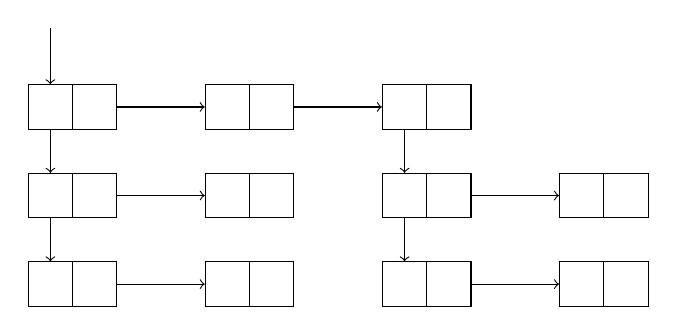
\begin{tikzpicture}[node distance = 0]
      % 0-0
      \node [box] (box-0-0-a) {};
      \node [box, right of = box-0-0-a, xshift = 16] (box-0-0-b) {};
      % 0-1
      \node [box, below of = box-0-0-a, yshift = -32] (box-0-1-a) {};
      \node [box, right of = box-0-1-a, xshift = 16] (box-0-1-b) {};
      % 0-2
      \node [box, below of = box-0-1-a, yshift = -32] (box-0-2-a) {};
      \node [box, right of = box-0-2-a, xshift = 16] (box-0-2-b) {};
      % 1-0
      \node [box, right of = box-0-0-b, xshift = 48] (box-1-0-a) {};
      \node [box, right of = box-1-0-a, xshift = 16] (box-1-0-b) {};
      % 1-1
      \node [box, right of = box-0-1-b, xshift = 48] (box-1-1-a) {};
      \node [box, right of = box-1-1-a, xshift = 16] (box-1-1-b) {};
      % 1-2
      \node [box, right of = box-0-2-b, xshift = 48] (box-1-2-a) {};
      \node [box, right of = box-1-2-a, xshift = 16] (box-1-2-b) {};
      % 2-0
      \node [box, right of = box-1-0-b, xshift = 48] (box-2-0-a) {};
      \node [box, right of = box-2-0-a, xshift = 16] (box-2-0-b) {};
      % 2-1
      \node [box, below of = box-2-0-a, yshift = -32] (box-2-1-a) {};
      \node [box, right of = box-2-1-a, xshift = 16] (box-2-1-b) {};
      % 2-2
      \node [box, below of = box-2-1-a, yshift = -32] (box-2-2-a) {};
      \node [box, right of = box-2-2-a, xshift = 16] (box-2-2-b) {};
      % 3-1
      \node [box, right of = box-2-1-b, xshift = 48] (box-3-1-a) {};
      \node [box, right of = box-3-1-a, xshift = 16] (box-3-1-b) {};
      % 3-2
      \node [box, right of = box-2-2-b, xshift = 48] (box-3-2-a) {};
      \node [box, right of = box-3-2-a, xshift = 16] (box-3-2-b) {};
     
      \draw [->] (0, 1) -- (box-0-0-a);
      \draw [->] (box-0-0-a) -- (box-0-1-a);
      \draw [->] (box-0-0-b) -- (box-1-0-a);
      \draw [->] (box-0-1-a) -- (box-0-2-a);
      \draw [->] (box-0-1-b) -- (box-1-1-a);
      \draw [->] (box-0-2-b) -- (box-1-2-a);
      \draw [->] (box-1-0-b) -- (box-2-0-a);
      \draw [->] (box-2-0-a) -- (box-2-1-a);
      \draw [->] (box-2-1-a) -- (box-2-2-a);
      \draw [->] (box-2-1-b) -- (box-3-1-a);
      \draw [->] (box-2-2-b) -- (box-3-2-a);
    \end{tikzpicture}
    \caption{}
  \end{subfigure}
  \begin{subfigure}{0.49\textwidth}
    \center
    \begin{tikzpicture}[node distance = 0]
      % 0-0
      \node [box] (box-0-0-a) {};
      \node [box, right of = box-0-0-a, xshift = 16] (box-0-0-b) {};
      % 0-1
      \node [box, below of = box-0-0-a, yshift = -48] (box-0-1-a) {};
      \node [box, right of = box-0-1-a, xshift = 16] (box-0-1-b) {};
      % 0-2
      \node [box, below of = box-0-1-a, yshift = -48] (box-0-2-a) {};
      \node [box, right of = box-0-2-a, xshift = 16] (box-0-2-b) {};
      % 1-0
      \node [box, right of = box-0-0-b, xshift = 48] (box-1-0-a) {};
      \node [box, right of = box-1-0-a, xshift = 16] (box-1-0-b) {};
      % 1-1
      \node [box, right of = box-0-1-b, xshift = 48] (box-1-1-a) {};
      \node [box, right of = box-1-1-a, xshift = 16] (box-1-1-b) {};
      % 1-2
      \node [box, right of = box-0-2-b, xshift = 48] (box-1-2-a) {};
      \node [box, right of = box-1-2-a, xshift = 16] (box-1-2-b) {};
      % 2-0
      \node [box, right of = box-1-0-b, xshift = 48] (box-2-0-a) {};
      \node [box, right of = box-2-0-a, xshift = 16] (box-2-0-b) {};

      \draw [->] (0, 1) -- (box-0-0-a);
      % 0-0
      \draw [->] (box-0-0-a) -- (box-0-1-a);
      \draw [->] (box-0-0-b) -- (box-1-0-a);
      % 0-1
      \draw [->] (box-0-1-a) -- (box-0-2-a);
      \draw [->] (box-0-1-b) -- (box-1-1-a);
      % 0-2
      \draw [->] (box-0-2-b) -- (box-1-2-a);
      % 1-0
      \draw [->] (box-1-0-b) -- (box-2-0-a);
      % 2-0
      \draw [->] (box-2-0-a) -- +(0, -0.8) -- +(-5, -0.8) -- +(-5, -1.7) --
      (box-0-1-a);
    \end{tikzpicture}
    \caption{}
  \end{subfigure}
  \begin{subfigure}{0.49\textwidth}
    \center
    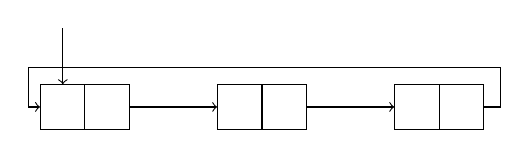
\begin{tikzpicture}[node distance = 0]
      % 0-0
      \node [box] (box-0-0-a) {};
      \node [box, right of = box-0-0-a, xshift = 16] (box-0-0-b) {};
      % 1-0
      \node [box, right of = box-0-0-b, xshift = 48] (box-1-0-a) {};
      \node [box, right of = box-1-0-a, xshift = 16] (box-1-0-b) {};
      % 2-0
      \node [box, right of = box-1-0-b, xshift = 48] (box-2-0-a) {};
      \node [box, right of = box-2-0-a, xshift = 16] (box-2-0-b) {};

      \draw [->] (0, 1) -- (box-0-0-a);
      \draw [->] (box-0-0-b) -- (box-1-0-a);
      \draw [->] (box-1-0-b) -- (box-2-0-a);
      \draw [->] (box-2-0-b) -- +(0.5, 0) -- +(0.5, 0.5) -- +(-5.5, 0.5) --
      +(-5.5, 0) -- (box-0-0-a);
    \end{tikzpicture}
    \caption{}
  \end{subfigure}
  \caption{}
\end{figure}

It is permitted for a substructure to occur in more than one place in a list
structure, as in Figure 1b, but it is not permitted for a structure to have
cycles, as in Figure 1c. An atomic symbol is represented in the computer by a
list structure of special form called the $
association\footnote{association$^*$: $noun$ an official group of people who
  have joined together for a particular purpose. $syn$ organization}
list$ of the symbol. The
address field of the first word contains a special
constant\footnote{constant$^*$: $adj.$ happening all the time or
  repeatedly. $noun$ (technical) a number or quantity that not vary. $opp$
  variable}
which enables the
program to tell that this word represents an atomic symbol. We shall describe
association lists in section 4b.

An S-expression $x$ that is not atomic is represented by a word, the address and
decrement parts of which contain the locations of the subexpressions $car[x]$
and $cdr[x]$, respectively. If we use the symbols $A$, $B$, etc. to denote the
locations of the association list of these symbols, then the S-expression $((A
\cdot B) \cdot (C \cdot (E \cdot F)))$ is represented by the list structure $a$
of Figure 2. Turning to the list form of S-expressions, we see that the
S-expression $(A, (B, C), D)$, which is an abbreviation for $(A \cdot ((B \cdot
(C \cdot NIL)) \cdot (D \cdot NIL)))$, is represented by the list structure of
Figure 2b.

\begin{figure}[h]
  \begin{subfigure}{0.49\textwidth}
    \center
    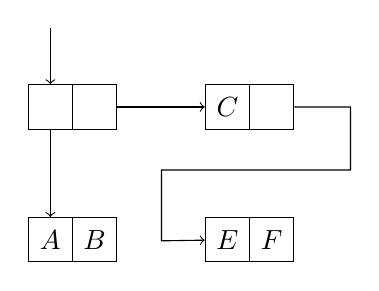
\begin{tikzpicture}[node distance = 0]
      % 0-0
      \node [box] (box-0-0-a) {};
      \node [box, right of = box-0-0-a, xshift = 16] (box-0-0-b) {};
      % 0-1
      \node [box, below of = box-0-0-a, yshift = -48] (box-0-1-a) {$A$};
      \node [box, right of = box-0-1-a, xshift = 16] (box-0-1-b) {$B$};
      % 1-0
      \node [box, right of = box-0-0-b, xshift = 48] (box-1-0-a) {$C$};
      \node [box, right of = box-1-0-a, xshift = 16] (box-1-0-b) {};
      % 1-1
      \node [box, right of = box-0-1-b, xshift = 48] (box-1-1-a) {$E$};
      \node [box, right of = box-1-1-a, xshift = 16] (box-1-1-b) {$F$};

      \draw [->] (0, 1) -- (box-0-0-a);
      \draw [->] (box-0-0-a) -- (box-0-1-a);
      \draw [->] (box-0-0-b) -- (box-1-0-a);
      \draw [->] (box-1-0-b) -- +(1, 0) -- +(1, -0.8) -- +(-1.4, -0.8) --
      +(-1.4, -1.7) -- (box-1-1-a);
    \end{tikzpicture}
    \caption{}
  \end{subfigure}
  \begin{subfigure}{0.49\textwidth}
    \center
    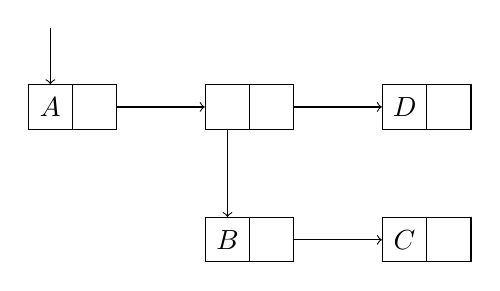
\begin{tikzpicture}[node distance = 0]
      % 0-0
      \node [box] (box-0-0-a) {$A$};
      \node [box, right of = box-0-0-a, xshift = 16] (box-0-0-b) {};
      % 1-0
      \node [box, right of = box-0-0-b, xshift = 48] (box-1-0-a) {};
      \node [box, right of = box-1-0-a, xshift = 16] (box-1-0-b) {};
      % 1-1
      \node [box, below of = box-1-0-a, yshift = -48] (box-1-1-a) {$B$};
      \node [box, right of = box-1-1-a, xshift = 16] (box-1-1-b) {};
      % 2-0
      \node [box, right of = box-1-0-b, xshift = 48] (box-2-0-a) {$D$};
      \node [box, right of = box-2-0-a, xshift = 16] (box-2-0-b) {};
      % 2-1
      \node [box, right of = box-1-1-b, xshift = 48] (box-2-1-a) {$C$};
      \node [box, right of = box-2-1-a, xshift = 16] (box-2-1-b) {};

      \draw [->] (0, 1) -- (box-0-0-a);
      \draw [->] (box-0-0-b) -- (box-1-0-a);
      \draw [->] (box-1-0-a) -- (box-1-1-a);
      \draw [->] (box-1-0-b) -- (box-2-0-a);
      \draw [->] (box-1-1-b) -- (box-2-1-a);
    \end{tikzpicture}
    \caption{}
  \end{subfigure}
  \caption{}
\end{figure}

When a list structure is regarded as representing a list, we see that each term
of the list
occupies\footnote{occupy$^*$: $verb$ \textit{occupy something} to fill or use a
  space, an area or an amount of time. $syn$ take up}
the address part of a word, the decrement part of which
$points$ to the word containing the next term, while the last word has $NIL$ in
its decrement.

An expression that has a given subexpression occurring more than once can be
represented in more than one way. Whether the list structure for the
subexpression is or not repeated depends upon the history of the
program. Whether or not a subexpression is repeated will make no difference in
the results of a program as they appear outside the machine, although it will
affect the time and storage requirements. For example, the S-expression $((A
\cdot B) \cdot (A \cdot B))$ can be represented by either the list structure of
Figure 3a or 3b.

\begin{figure}[h]
  \begin{subfigure}{0.49\textwidth}
    \center
    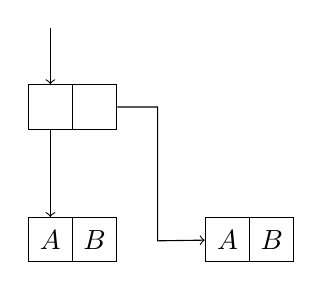
\begin{tikzpicture}[node distance = 0]
      \node [box] (box-0-0-a) {};
      \node [box, right of = box-0-0-a, xshift = 16] (box-0-0-b) {};
      \node [box, below of = box-0-0-a, yshift = -48] (box-0-1-a) {$A$};
      \node [box, right of = box-0-1-a, xshift = 16] (box-0-1-b) {$B$};
      \node [box, right of = box-0-1-b, xshift = 48] (box-1-1-a) {$A$};
      \node [box, right of = box-1-1-a, xshift = 16] (box-1-1-b) {$B$};

      \draw [->] (0, 1) -- (box-0-0-a);
      \draw [->] (box-0-0-a) -- (box-0-1-a);
      \draw [->] (box-0-0-b) -- +(0.8, 0) -- +(0.8, -1.7) -- (box-1-1-a);
    \end{tikzpicture}
    \caption{}
  \end{subfigure}
  \begin{subfigure}{0.49\textwidth}
    \center
    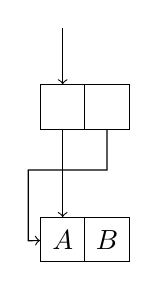
\begin{tikzpicture}[node distance = 0]
      \node [box] (box-0-0-a) {};
      \node [box, right of = box-0-0-a, xshift = 16] (box-0-0-b) {};
      \node [box, below of = box-0-0-a, yshift = -48] (box-0-1-a) {$A$};
      \node [box, right of = box-0-1-a, xshift = 16] (box-0-1-b) {$B$};

      \draw [->] (0, 1) -- (box-0-0-a);
      \draw [->] (box-0-0-a) -- (box-0-1-a);
      \draw [->] (box-0-0-b) -- +(0, -0.8) -- +(-1, -0.8) -- +(-1, -1.7) --
      (box-0-1-a);
    \end{tikzpicture}
    \caption{}
  \end{subfigure}
  \caption{}
\end{figure}

The
prohibition\footnote{prohibition: $noun$ 1. (formal) the act of stopping
  something being done or used, especially by law. 2. \textit{prohibition
    (against/on something)} (formal) a law or a rule that stop something to be
  done or used.}
against circular list structures is essentially a prohibition
against an expression being a subexpression of itself. Such an expression could
not exist on paper in a world with our
topology\footnote{topology: $noun$ (technical) the way, the part of something
  are arranged and related.}.
Circular list structures would
have some advantages in the machine, for example, for representing recursive
functions, but difficulties in printing them, and in certain other operations,
make it seem advisable not to use them for the present.

The advantages of list structures for the storage of symbolic expressions are:
\begin{enumerate}
\item The size and even the number of expressions with which the program will
  have to deal cannot be predicted in advance. Therefore, it is difficult to
  arrange blocks of storage of fixed length to contain them.
\item Registers can be put back on the free-storage list when they are no longer
  needed. Even one register returned to the list is of value, but if expressions
  are stored linearly, it is difficult to make use of blocks of registers of odd
  sizes that may become available.
\item An expression that occurs as a subexpression of several expressions need
  be represented in storage only once.
\end{enumerate}

\paragraph{b.}\textit{Association Lists.}
In the LISP programming system we put more in the association list of a symbol
than is required by the mathematical system described in the previous
sections. In fact, any information that we desire to may include: the $print
\ name$, that is, the string of letters and digits which represents the symbol
outside the machine; a
numerical\footnote{numerical: $adj.$ relating to numbers; expressed in numbers.}
value if the symbol represents a number;
another S-expression if the symbol, in some way, serves as a name for it; or the
location of a
routine\footnote{routine$^*$: $noun$ the normal order and way in which you
  regularly do things.}
if the symbol represents a function for which there is a
machine-language subroutine. All this implies that in the machine system there
are more primitive entities than have been described in the sections on the
mathematical system.

For the present, we shall only describe how $print \ names$ are presented on
association lists so that in reading or printing the program can
establish\footnote{establish$^*$: $verb$ \textit{establish something} to start
  or create an organization, a system, etc. that is meant to last for a long
  time. $syn$ set up}
a
correspondence between information on punched cards,
magnetic\footnote{magnetic: $adj.$ be having like a magnet. --- magnet: $noun$ a
  piece of iron that attracts objects made of iron towards it, either naturally
  or because of electric current that is passed through it. ------attract:
  $verb$ if you are attracted by something, it interests you and makes you want
  it; if you are attracted by somebody, you like or admire them.}
tape or printed
page and the list structure inside the machine. The association list of the
symbol $DIFFERENTIATE$ has a segment of the form shown in Figure 4. Here $pname$
is a symbol that indicates that the structure for the print name of the symbol
whose association list this is hanging from the next word on the association
list. In the second row of the figure we have a list of three words. The address
part of each of these words points to a Word containing six 6-bit
characters. The last word is filled out with a 6-bit combination that does not
represent a character printable by the computer. (Recall that the IBM 704 has a
36-bit word and that printable characters are each represented by 6-bits.) The
presence\footnote{presence$^*$: $noun$ the fact of being in a particular
  place. $opp$ absence}
of the words with character information means that the association
lists do not themselves represent S-expressions, and that only some of the
functions for dealing with S-expressions make sense within an association list.

\begin{figure}[h]
  \center
  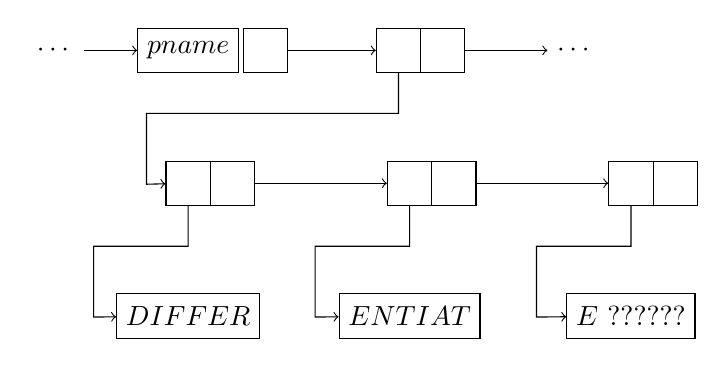
\begin{tikzpicture}[node distance = 0]
    % textarea-left
    \node [textarea] (textarea-left) {$\cdots$};
    % 0-0
    \node [box, below of = textarea-left, xshift = 48] (box-0-0-a) {$pname$};
    \node [box, right of = box-0-0-a, xshift = 28] (box-0-0-b) {};
    % 1-0
    \node [box, right of = box-0-0-b, xshift = 48] (box-1-0-a) {};
    \node [box, right of = box-1-0-a, xshift = 16] (box-1-0-b) {};
    % textarea-right
    \node [textarea, right of = box-1-0-b, xshift = 48] (textarea-right) {$\cdots$};
    % 0-1
    \node [box, below of = box-0-0-a, yshift = -48] (box-0-1-a) {};
    \node [box, right of = box-0-1-a, xshift = 16] (box-0-1-b) {};
    % 1-1
    \node [box, right of = box-0-1-b, xshift = 64] (box-1-1-a) {};
    \node [box, right of = box-1-1-a, xshift = 16] (box-1-1-b) {};
    % 2-1
    \node [box, right of = box-1-1-b, xshift = 64] (box-2-1-a) {};
    \node [box, right of = box-2-1-a, xshift = 16] (box-2-1-b) {};
    % 0-2
    \node [box, below of = box-0-1-a, yshift = -48] (box-0-2) {$DIFFER$};
    % 1-2
    \node [box, below of = box-1-1-a, yshift = -48] (box-1-2) {$ENTIAT$};
    % 2-2
    \node [box, below of = box-2-1-a, yshift = -48] (box-2-2) {$E \ ??????$};

    \draw [->] (textarea-left) -- (box-0-0-a);
    \draw [->] (box-0-0-b) -- (box-1-0-a);
    \draw [->] (box-1-0-a) -- +(0, -0.8) -- +(-3.2, -0.8) -- +(-3.2, -1.7) --
    (box-0-1-a);
    \draw [->] (box-1-0-b) -- (textarea-right);
    \draw [->] (box-0-1-a) -- +(0, -0.8) -- +(-1.2, -0.8) -- +(-1.2, -1.7) --
    (box-0-2);
    \draw [->] (box-0-1-b) -- (box-1-1-a);
    \draw [->] (box-1-1-a) -- +(0, -0.8) -- +(-1.2, -0.8) -- +(-1.2, -1.7) --
    (box-1-2);
    \draw [->] (box-1-1-b) -- (box-2-1-a);
    \draw [->] (box-2-1-a) -- +(0, -0.8) -- +(-1.2, -0.8) -- +(-1.2, -1.7) --
    (box-2-2);
  \end{tikzpicture}
  \caption{}
\end{figure}

\paragraph{c.}\textit{Free-storage List.}
At any given time only a part of the memory
reserved\footnote{reserve: $verb$ to ask for a seat, table, room, etc. to be
  available for you or somebody else at a future time. $syn$ book}
for list structures will
actually be in use for storing S-expressions. The remaining registers (in our
system the number, initially, is approximately 15,000) are arranged in a single
list called the $free-storage \ list$. A certain register, FREE, in the program
contains the location of the first register in this list. When a word is
required to form some additional list structure, the first word on the
$free-storage \ list$ is taken and the number in register FREE is changed to
become the location of the second word on the free-storage list. No
provision\footnote{provision: $noun$ the act of supplying somebody with
  something that they need or want; something that is supplied.}
need be made for the user to program the return of registers to the free-storage
list.

This return takes place automatically, approximately as follows (it is necessary
to give a simplified description of this process in this report); There is a
fixed set of base registers in the program which contains the locations of list
structures that are accessible to the program. Of course, because list
structures branch, an arbitrary number of registers may be involved. Each
register that is accessible to the program is accessible because it can be
reached from one or more of the base registers by a chain of $car$ and $cdr$
operations. When the contents of a base register are changed, it may happen that
the register to which the base register
formerly\footnote{formerly$^*$: $adv.$ in earlier time. $syn$ previously}
pointed cannot be reached by a
$car - cdr$ chain from any base register. Such a register may be considered
abandoned by the program because its contents can no longer be found by any
possible program;
hence\footnote{hence$^*$: $adv.$ (formal) for this reason.}
its contents are no longer of interest, and so we would
like to have it back on the free-storage list. This comes about in the following
way.

Nothing happens until the program runs out of the free-storage list. When a free
register is wanted, and there is none left on the free-storage list, a
reclamation\footnote{reclaim: $verb$ to get something back or to ask to have it
  back after it has been lost, taken away, etc.}
cycle starts.

First, the program finds all registers accessible from the base registers and
makes their signs negative. This is accomplished by starting from each of the
base registers and changing the sign of every register that can be reached from
it by a $car = cdr$ chain. If the program encounters a register in this process
which already has a negative sign, it assumes that this register has already
been reached.

After all of the accessible registers have had their signs changed, the program
goes through the area of memory reserved for the storage of list structures and
puts all the registers whose signs were not changed in the previous step back on
the free-storage list, and makes the signs of the accessible registers positive
again.

This process, because it is
entirely\footnote{entirely$^*$: $adv.$ in every way possible; completely.}
automatic, is more convenient for the
programmer than a system in which he has to keep
track\footnote{track$^*$: $noun$ a rough path or road, usually one that has not
  been built but that has been made by people walking there.}
of and erase unwanted
lists. Its
efficiency\footnote{efficiency: $noun$ the quality of doing something well with
  no waste of time or money.}
depends upon not coming close to
exhausting\footnote{exhaust: $noun$ wastes gases that come out of a vehicle, an
  engine or a machine. $verb$ 1. to make somebody feel very tired. $syn$ wear
  out 2. \textit{exhaust something} to use all of something so that there is
  none left.}
the available
memory with accessible lists. This is because the reclamation process requires
several seconds to execute, and therefore must result in the addition of at
least several thousand registers to the free-storage list if the program is not
to spend most of its time in reclamation.

\paragraph{d.}\textit{Elementary S-functions in the Computer.}
We shall now describe the computer representations of $atom$, $=$, $car$, $cdr$,
and $cons$. An S-expression in communicated to the program that represents a
function as the location of the word representing it, and the program give
S-expression answers in the same form.

$atom$. As stated above, a word representing an atomic symbol has a special
constant in its address part: $atom$ is programmed as an open subroutine that
tests this part. Unless the M-expression $atom[e]$ occurs as a condition in a
conditional expression, the symbol $T$ or $F$ is generated as the result of the
test. In case of a conditional expression, a conditional transfer is used and
the symbol $T$ or $F$ is not generated.

$eq$. The program for $eq[e;f]$ involves testing for the numerical equality of
the locations of the words. This works because each atomic symbol has only one
association list. As with $atom$, the result is either a conditional transfer or
one of the symbols $T$ or $F$.

$car$. Computing $car[x]$ involves getting the contents of the address part of
register $x$. This is essentially accomplished by the single instruction CLA 0,
i, where the argument is in index register, and the result appears in the
address part of the accumulator. (We take the view that the places from which a
function takes its arguments and into which it puts its results are
prescribed\footnote{prescribe: $verb$ 1. (of a doctor) to tell somebody to take
  a particular medicine or have a particular treatment; to write a PRESCRIPTION
  for a particular medicine. 2. (of a person or an organization with authority)
  to say what should be done or how something should be done. $syn$ stipulate}
in the definition of the function, and it is the
responsibility\footnote{responsibility$^*$: $noun$ a duty to deal with or take
  care of somebody/something, so that you may be blamed if something goes
  wrong. --- duty: $noun$ something that you feel you have to do because it is
  your moral or legal responsibility. ------ moral: $adj.$ concerned with
  principles of right and wrong behavior. $noun$ standards or principles of good
  behavior, especially in matters of sexual relationships. --------- principle:
  $noun$ a moral rule or a strong belief that influences your actions. ---
  blame: $verb$ to think or say that somebody/something is responsible for
  something bad.}
of the
programmer or the compiler to insert the required datamoving instructions to get
the results of one calculation in position for the next.)(``car'' is a mnemonic
for ``contents of the address part of register''.)

$cdr$. $cdr$ is handled in the same way as $car$, except that the result appears
in the decrement part of the accumulator. (``cdr'' stands for ``contents of the
decrement part of register''.)

$cons$. The value of $cons[x; y]$ must be the location of a register that has
$x$ and $y$ in its address and decrement part, respectively. There may not be
such a register in the computer and, even if there were, it would be
time-consuming\footnote{consume: $verb$ \textit{consume something} to use
  something, especially fuel, energy or time.}
to find it. Actually, what we do is to take the first available
register from the $free-storage \ list$, put $x$ and $y$ in the address and
decrement parts, respectively, and make the value of the function the location
of the register taken. (``cons'' is an abbreviation for ``construct''.)

It is the subroutine for $cons$ that initiates the reclamation when the
$free-storage \ list$ is exhausted. In the version of the system that is used at
present $cons$ is represented by closed subroutine. In the compiled version,
$cons$ is open.

\paragraph{e.}\textit{Representation of S-function by Programs.}
The
compilation\footnote{compilation: $noun$ a collection of items, especially
  pieces of music or writing, taken from different places and put together.}
of functions that are compositions of $car$, $cdr$, and $cons$,
either by hand or by a compiler program, is
straightforward\footnote{straightforward: $adj.$ easy to do or understand; not
  complicated. $syn$ easy}.
Conditional
expressions give no trouble except that they must be so compiled that only the
$p$'s and $e$'s that are required are computed. However, problems arise in the
compilation of recursive functions.

In general (we shall discuss an exception), the routine for a recursive function
uses itself as a subroutine. For example, the program for $subst[x; y; z]$ uses
itself as a subroutine to evaluate the result of substituting into the
subexpressions $car[z]$ and $cdr[z]$. While $subst[x; y; cdr[z]]$ is being
evaluated, the result of the previous evaluation of $subst[x; y; cdr[z]]$ must
be saved in a temporary storage register. However, $subst$ may need the same
register for evaluating $subst[x; y; cdr[z]]$. This possible conflict is
resolved by the SAVE and UNSAVE routines that use the $public \ push-down
\ list$. The SAVE routine is entered at the beginning of the routine for the
recursive function with a request to save a given set of
consecutive\footnote{consecutive: $adj.$ following one after another in a series
  with out interruption. --- interruption: $noun$ something that temporarily
  stops an activity or a situation; a time when an activity is stopped.}
registers. A block of registers called the $public \ push-down \ list$ is
reserved for this purpose The SAVE routine has an index that tells it how many
registers in the push-down list are already in use. It moves the contents of the
registers which are to be saved to the first unused registers in the push-down
list, advances the index of the list, and returns to the program from which
control came. This program may then freely use these registers for temporary
storage. Before the routine exits it use UNSAVE, which restores the contents of
the temporary registers from the push-down list and moves back the index of this
list. The result of these conventions is described, in programming
terminology\footnote{terminology: $noun$ the set of technical words or
  expressions used in a particular subject.},
by saying that the recursive subroutine is
transparent\footnote{transparent$^*$: $adj.$ (of glass, plastic, etc.) allowing
  you to see through it. $opp$ opaque}
to the temporary storage
registers.

\paragraph{f.}\textit{Status of the LISP Programming System (February 1960).}
A
variant\footnote{variant: $noun$ \textit{variant (of/on something)} a change,
  especially in the amount or level of something.}
of the function apply described in section 5f has been translated into
a program APPLY for the IBM 704. Since this routine can compute values of
S-functions given their descriptions as S-expressions and their arguments, it
serves as an interpreter for the LISP programming language which describes
computation processes in this way.

The program APPLY has been imbedded in the LISP programming system which has the
following features:
\begin{enumerate}
\item The programmer may define any number of S-functions by
  S-expressions. These functions may refer to each other or to certain
  S-functions represented by machine language program.
\item The values of defined functions may be computed.
\item S-expressions may be read and printed (directly or via magnetic tape).
\item Some error
  diagnostic\footnote{diagnostic: $adj.$ (technical) connected with identifying
    something, especially an illness. $noun$ 1. (computing) a program used for
    identifying a computer fault. 2. a message on a computer screen giving
    information about a fault. --- identify: $verb$ to recognize
    somebody/something and be able to say who or what they are.}
  and selective tracing facilities are included.
\item The programmer and selected S-functions compiled into machine language
  programs put into the core memory. Values of compiled functions are computed
  about 60 times as fast as they would if interpreted. Compilation is fast
  enough so that it is not necessary to punch compiled program for future use.
\item A ``program feature'' allows programs containing assignment and \textbf{go
  to} statements in the style of ALGOL.
\item Computation with floating point numbers is possible in the system, but
  this is inefficient.
\item A programmer's
  manual\footnote{manual: $adj.$ (of work, etc.) involving using the hands or
    physical strength. $noun$ a book that tells you how to do or operate
    something, especially one that comes with a machine, etc. when you buy it.}
  is being prepared. The LISP programming system is
  appropriate for computations where the data can conveniently be represented as
  symbolic expressions allowing expressions of the same kind as
  subexpressions. A version of the system for the IBM 709 is being prepared.
\end{enumerate}

\section{Another Formalism for Functions of Symbolic Expressions}

There are a number of ways of defining functions of symbolic expressions which
are quite similar to the system we have adopted. Each of them involves three
basic functions, conditional expressions, and recursive function definitions,
but the class of expressions corresponding to S-expressions is different, and so
are the precise definitions of the functions. We shall describe one of these
variants called linear LISP.

The L-expressions are defined as follows:
\begin{enumerate}
\item A finite list of characters is admitted.
\item Any string of admitted characters in an L-expression. This includes the
  null string denoted by $\Lambda$.
\end{enumerate}

There are three functions of strings:
\begin{enumerate}
\item $first[x]$ is the first character of the string $x$.

  $first[\Lambda]$ is undefined. For example: $first[ABC] = A$.
\item $rest[x]$ is the string of characters which remains when the first
  character of the string is deleted.

  $rest[\Lambda]$ is undefined. For example: $rest[ABC] = BC$.
\item $combine[x; y]$ is the string formed by prefixing the character $x$ to the
  string $y$. For example: $combine[A; BC] = ABC$.
\end{enumerate}

There are three predicates on strings:
\begin{enumerate}
\item $char[x]$, $x$ is a single character.
\item $null[x]$, $x$ is a null string.
\item $x = y$, defined for $x$ and $y$ characters.
\end{enumerate}

The advantage of linear LISP is that no characters are given special roles, as
are parentheses, dots, and commas in LISP. This permits computations with all
expressions that can be written linearly. The disadvantage of linear LISP is
that the
extraction\footnote{extraction: $noun$ the act or process of removing or
  obtaining something from something else.}
of subexpressions is a fairly involved, rather than an
elementary, operation. It is not hard to write, in linear LISP, functions that
correspond to the basic functions of LISP, so that, mathematically, linear LISP
includes LISP. This turns out to be the most convenient way of programming, in
linear LISP, the most complicated manipulations. However, if the functions are
to be represented by computer routines, LISP is essentially faster.

\section{Flowcharts and Recursion}

Since both the usual form of computer program and recursive function definitions
are universal computationally, it is interesting to display the relation between
them. The translation of recursive symbolic functions into computer programs was
the subject of the rest of this report. In this section we show how to go the
other way, at list in principle.

The state to the machine at any time during a computation is given by the values
of a number of variables. Let these variables be combined into a vector
$\xi$. Consider a program block with one
entrance\footnote{entrance$^*$: $noun$ \textit{entrance (to something)} a door,
  gate, passage, etc. used for entering a room, building or place.}
and one exit. It defines and
is essentially defined by a certain function $f$ that takes one machine
configuration into another, that is, $f$ has the form $\xi' = f(\xi)$. Let us
call $f$ the associated function of the program block. Now let a number of such
blocks be combined into a program by decision element $\pi$ that decide after
each block is completed which block will be entered next. Nevertheless, let the
whole program still have one entrance and one exit.

\begin{figure}[h]
  \center
  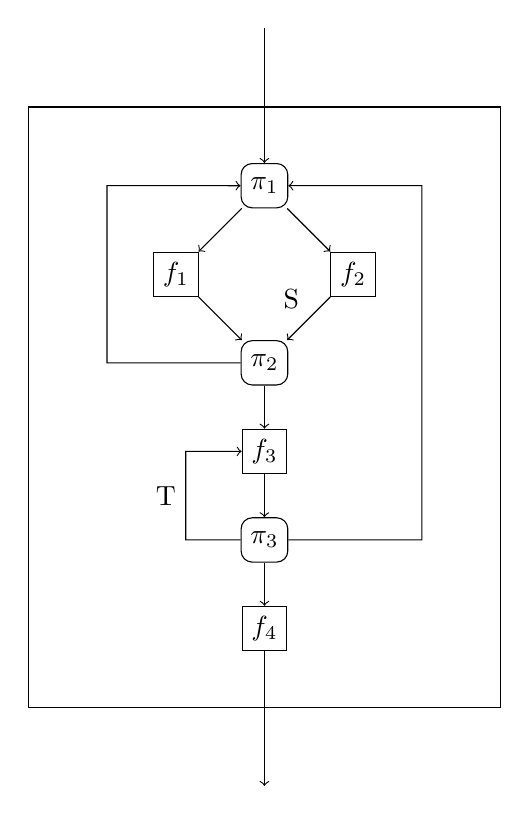
\begin{tikzpicture}[node distance = 0]
    \node [pi] (pi-1) {$\pi_1$};
    \node [box, below of = pi-1, yshift = -32, xshift = -32] (f-1) {$f_1$};
    \node [box, below of = pi-1, yshift = -32, xshift = 32] (f-2) {$f_2$};
    \node [pi, below of = pi-1, yshift = -64] (pi-2) {$\pi_2$};
    \node [box, below of = pi-2, yshift = -32] (f-3) {$f_3$};
    \node [pi, below of = f-3, yshift = -32] (pi-3) {$\pi_3$};
    \node [box, below of = pi-3, yshift = -32] (f-4) {$f_4$};

    \draw [->] (0, 2) -- (pi-1);
    \draw [->] (pi-1) -- (f-1);
    \draw [->] (pi-1) -- (f-2);
    \draw [->] (f-1) -- (pi-2);
    \draw [->] (f-2) -- node[anchor = south east] {S} (pi-2);
    \draw [->] (pi-2) -- (f-3);
    \draw [->] (pi-2) -- +(-2, 0) -- +(-2, 2.25) -- (pi-1);
    \draw [->] (f-3) -- (pi-3);
    \draw [->] (pi-3) -- (f-4);
    \draw [->] (pi-3) -- +(2, 0) -- +(2, 4.5) -- (pi-1);
    \draw [->] (pi-3) -- +(-1, 0) -- node[anchor = east] {T} +(-1, 1.125) -- (f-3);
    \draw [->] (f-4) -- +(0, -2);
    \draw [-] (3, 1) -- (3, -6.63) -- (-3, -6.63) -- (-3, 1) -- (3, 1);
  \end{tikzpicture}
  \caption{}
\end{figure}

We give as an example the flowchart of figure 5. Let us describe the function
$r[\xi]$ that gives the
transformation\footnote{transformation: $noun$ a complete change in
  somebody/something}.
of the vector $\xi$ between entrance and
exit of the whole block. We shall define it in conjunction with the functions
$s(\xi)$, and $t{\xi}$, which give the transformations that $\xi$ undergoes
between the points S and T, respectively, and the exit. We have
\begin{align*}
  r[\xi] &= [\pi_11[\xi] \to S[f1[\xi]]; T \to S[f_2[\xi]]] \\
  S[\xi] &= [\pi_21[\xi] \to r[\xi]; T \to t[f_3[\xi]]]     \\
  t[\xi] &= [\pi_31[\xi] \to f_4[\xi]; \pi_32[\xi] \to r[\xi]; T \to
    t[f_3[\xi]]]
\end{align*}

Given a flowchart with a single entrance and a single exit, it is easy to write
down the recursive function that gives the transformation of the state vector
from entrance to exit in terms of the corresponding functions for the
computation blocks and the predicates of the branch. In general, we proceed as
follows.

In figure 6, let $\beta$ be an n-way branch point, and let $f_1, \ldots, f_n$ be
the computations leading to branch points $\beta_1, \beta_2, \ldots,
\beta_n$. Let $\phi$ be the function that transforms $\xi$ between $beta$ and
the exit of the chart, and let $\phi_1, \ldots, \phi_n$ be the corresponding
functions for $\beta_1, \ldots, \beta_n$. We then write
$$ \phi[\xi] = [p_1[\xi] \to \phi_1[f_1[\xi]]; \ldots; p_n[\xi] \to
  \phi_n[\xi]] $$

\begin{figure}[h]
  \center
  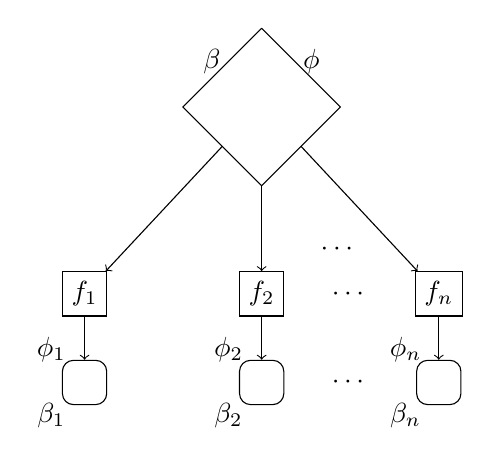
\begin{tikzpicture}[node distance = 0]
    \draw [-] (0, 0) -- (-1, -1) -- (0, -2) -- (1, -1) -- (0, 0);
    \node [box, xshift = -64, yshift = -96] (f-1) {$f_1$};
    \node [box, xshift = 0, yshift = -96] (f-2) {$f_2$};
    \node [box, xshift = 64, yshift = -96] (f-n) {$f_n$};
    \node [pi, below of = f-1, yshift = -32] (pi-1) {};
    \node [pi, below of = f-2, yshift = -32] (pi-2) {};
    \node [pi, below of = f-n, yshift = -32] (pi-n) {};
    \draw [->] (-0.5, -1.5) -- (f-1);
    \draw [->] (0, -2) -- (f-2);
    \draw [->] (0.5, -1.5) -- (f-n);
    \draw [->] (f-1) -- (pi-1);
    \draw [->] (f-2) -- (pi-2);
    \draw [->] (f-n) -- (pi-n);
    \draw node[left of = f-n, xshift = -36, yshift = 16] {$\cdots$};
    \draw node[left of = f-n, xshift = -32] {$\cdots$};
    \draw node[left of = pi-n, xshift = -32] {$\cdots$};
    \draw node[xshift = -18, yshift = -12] {$\beta$};
    \draw node[xshift = 18, yshift = -12] {$\phi$};
    \draw node[above of = pi-1, xshift = -12, yshift = 12] {$\phi_1$};
    \draw node[below of = pi-1, xshift = -12, yshift = -12] {$\beta_1$};
    \draw node[above of = pi-2, xshift = -12, yshift = 12] {$\phi_2$};
    \draw node[below of = pi-2, xshift = -12, yshift = -12] {$\beta_2$};
    \draw node[above of = pi-n, xshift = -12, yshift = 12] {$\phi_n$};
    \draw node[below of = pi-n, xshift = -12, yshift = -12] {$\beta_n$};
  \end{tikzpicture}
  \caption{}
\end{figure}

\section {Acknowledgments}
The inadequacy of the $\lambda$ for naming recursive functions was noticed by
N.Rochester, and he discovered an alternative to the solution involving $label$
which has been used here. The form of subroutine for $cons$ which permits its
composition with other functions was invented, in connection with another
programming system, by C.Gerberick and H.L.Gelernter, of IBM Corporation. The
LISP programming system was developed by a group including R.Brayton, D.Edwards,
P.Fox, L.Hodes, D.Luckham, K.Maling, J.McCarthy, D.Park, S.Russell.

The group was supported by the M.I.T. Computation Center, and by the
M.I.T. Research Laboratory of Electronics (which is supported in part by the
U.S. Army (Signal Corps), the U.S. Air Force (Office of Scientific Research, Air
Research and Development Command), and the U.S.Navy (Office of Naval
Research)). The author also wishes to acknowledge the personal financial support
of the Alfred P.Sloan Foundation.

% ~\cite{McCarthy1958}
% ~\cite{Newell1957}
% ~\cite{Church1941}
% ~\cite{FORTRAN1956}
% ~\cite{Perlis1958}

\bibliographystyle{unsrt}
\bibliography{references}

\end{document}
